\documentclass{standalone}
\usepackage{tikz}
\usetikzlibrary{patterns, positioning}


\begin{document}
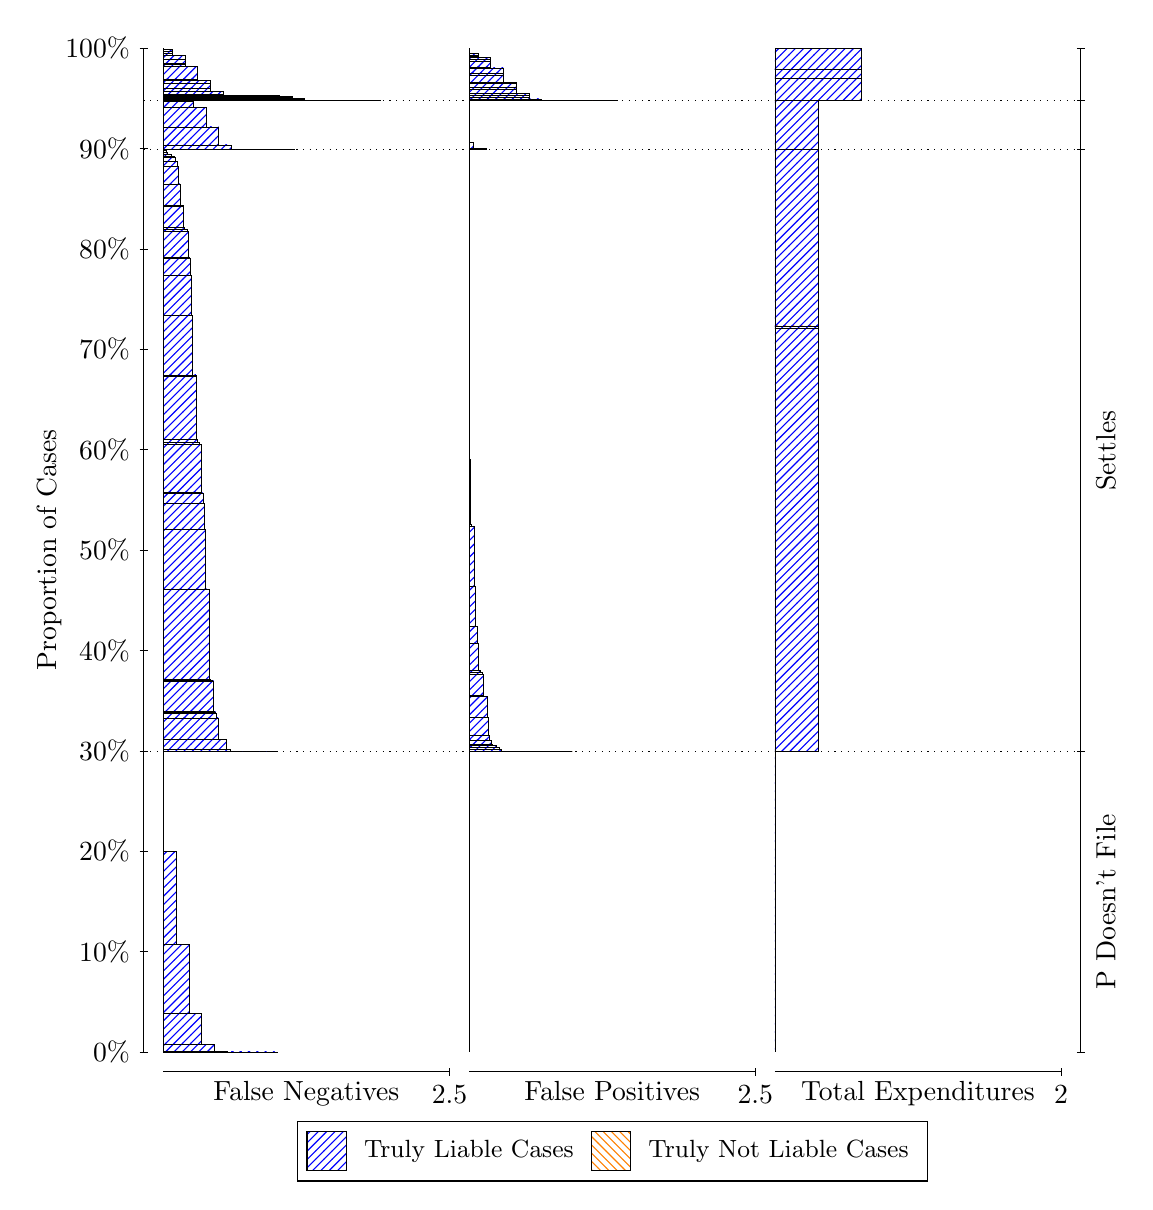
\begin{tikzpicture}
\draw[black, very thin] (1.5,1.75) -- (1.5,14.5);
\node[rotate=90, text=black, anchor=center] at (0.3, 8.125) {Proportion of Cases};
\draw[black, very thin] (1.45,1.75) -- (1.55,1.75);
\node[text=black, anchor=east] at (1.45, 1.75) {0\%};
\draw[black, very thin] (1.45,3.025) -- (1.55,3.025);
\node[text=black, anchor=east] at (1.45, 3.025) {10\%};
\draw[black, very thin] (1.45,4.3) -- (1.55,4.3);
\node[text=black, anchor=east] at (1.45, 4.3) {20\%};
\draw[black, very thin] (1.45,5.575) -- (1.55,5.575);
\node[text=black, anchor=east] at (1.45, 5.575) {30\%};
\draw[black, very thin] (1.45,6.85) -- (1.55,6.85);
\node[text=black, anchor=east] at (1.45, 6.85) {40\%};
\draw[black, very thin] (1.45,8.125) -- (1.55,8.125);
\node[text=black, anchor=east] at (1.45, 8.125) {50\%};
\draw[black, very thin] (1.45,9.4) -- (1.55,9.4);
\node[text=black, anchor=east] at (1.45, 9.4) {60\%};
\draw[black, very thin] (1.45,10.675) -- (1.55,10.675);
\node[text=black, anchor=east] at (1.45, 10.675) {70\%};
\draw[black, very thin] (1.45,11.95) -- (1.55,11.95);
\node[text=black, anchor=east] at (1.45, 11.95) {80\%};
\draw[black, very thin] (1.45,13.225) -- (1.55,13.225);
\node[text=black, anchor=east] at (1.45, 13.225) {90\%};
\draw[black, very thin] (1.45,14.5) -- (1.55,14.5);
\node[text=black, anchor=east] at (1.45, 14.5) {100\%};

\draw[black, very thin] (13.4,1.75) -- (13.4,14.5);
\draw[black, very thin] (13.35,1.75) -- (13.45,1.75);
\node[anchor=west] at (13.35, 1.75) {};
\draw[black, very thin] (13.35,5.563) -- (13.45,5.563);
\node[anchor=west] at (13.35, 5.563) {};
\draw[black, very thin] (13.35,13.21) -- (13.45,13.21);
\node[anchor=west] at (13.35, 13.21) {};
\draw[black, very thin] (13.35,13.833) -- (13.45,13.833);
\node[anchor=west] at (13.35, 13.833) {};
\draw[black, very thin] (13.35,14.5) -- (13.45,14.5);
\node[anchor=west] at (13.35, 14.5) {};

\draw[black, very thin, pattern color=blue, pattern=north east lines] (1.75,1.75) rectangle (3.2033,1.75);
\draw[black, very thin, pattern color=blue, pattern=north east lines] (1.75,1.75) rectangle (3.0419,1.75);
\draw[black, very thin, pattern color=blue, pattern=north east lines] (1.75,1.75) rectangle (2.8804,1.75);
\draw[black, very thin, pattern color=blue, pattern=north east lines] (1.75,1.75) rectangle (2.7189,1.7503);
\draw[black, very thin, pattern color=blue, pattern=north east lines] (1.75,1.7503) rectangle (2.5574,1.7582);
\draw[black, very thin, pattern color=blue, pattern=north east lines] (1.75,1.7582) rectangle (2.3959,1.8434);
\draw[black, very thin, pattern color=blue, pattern=north east lines] (1.75,1.8434) rectangle (2.2344,2.2366);
\draw[black, very thin, pattern color=blue, pattern=north east lines] (1.75,2.2366) rectangle (2.073,3.1157);
\draw[black, very thin, pattern color=blue, pattern=north east lines] (1.75,3.1157) rectangle (1.9115,4.2995);
\draw[black, very thin, pattern color=orange, pattern=north west lines] (1.75,4.2995) rectangle (1.75,4.2995);
\draw[black, very thin, pattern color=blue, pattern=north east lines] (1.75,4.2995) rectangle (1.75,5.563);
\draw[black, very thin, pattern color=blue, pattern=north east lines] (1.75,5.563) rectangle (3.2033,5.563);
\draw[black, very thin, pattern color=blue, pattern=north east lines] (1.75,5.563) rectangle (3.1307,5.563);
\draw[black, very thin, pattern color=blue, pattern=north east lines] (1.75,5.563) rectangle (3.058,5.563);
\draw[black, very thin, pattern color=blue, pattern=north east lines] (1.75,5.563) rectangle (3.0419,5.563);
\draw[black, very thin, pattern color=blue, pattern=north east lines] (1.75,5.563) rectangle (2.9853,5.563);
\draw[black, very thin, pattern color=blue, pattern=north east lines] (1.75,5.563) rectangle (2.9692,5.563);
\draw[black, very thin, pattern color=blue, pattern=north east lines] (1.75,5.563) rectangle (2.9127,5.563);
\draw[black, very thin, pattern color=blue, pattern=north east lines] (1.75,5.563) rectangle (2.8965,5.563);
\draw[black, very thin, pattern color=blue, pattern=north east lines] (1.75,5.563) rectangle (2.8804,5.563);
\draw[black, very thin, pattern color=blue, pattern=north east lines] (1.75,5.563) rectangle (2.8239,5.563);
\draw[black, very thin, pattern color=blue, pattern=north east lines] (1.75,5.563) rectangle (2.8077,5.563);
\draw[black, very thin, pattern color=blue, pattern=north east lines] (1.75,5.563) rectangle (2.7673,5.5641);
\draw[black, very thin, pattern color=blue, pattern=north east lines] (1.75,5.5641) rectangle (2.7512,5.5641);
\draw[black, very thin, pattern color=blue, pattern=north east lines] (1.75,5.5641) rectangle (2.735,5.5641);
\draw[black, very thin, pattern color=blue, pattern=north east lines] (1.75,5.5641) rectangle (2.7189,5.5641);
\draw[black, very thin, pattern color=blue, pattern=north east lines] (1.75,5.5641) rectangle (2.6947,5.5642);
\draw[black, very thin, pattern color=blue, pattern=north east lines] (1.75,5.5642) rectangle (2.6624,5.5642);
\draw[black, very thin, pattern color=blue, pattern=north east lines] (1.75,5.5642) rectangle (2.6462,5.5642);
\draw[black, very thin, pattern color=blue, pattern=north east lines] (1.75,5.5642) rectangle (2.6059,5.5943);
\draw[black, very thin, pattern color=blue, pattern=north east lines] (1.75,5.5943) rectangle (2.5897,5.5968);
\draw[black, very thin, pattern color=blue, pattern=north east lines] (1.75,5.5968) rectangle (2.5736,5.5972);
\draw[black, very thin, pattern color=blue, pattern=north east lines] (1.75,5.5972) rectangle (2.5574,5.5974);
\draw[black, very thin, pattern color=blue, pattern=north east lines] (1.75,5.5974) rectangle (2.5493,5.7195);
\draw[black, very thin, pattern color=blue, pattern=north east lines] (1.75,5.7195) rectangle (2.5332,5.7197);
\draw[black, very thin, pattern color=blue, pattern=north east lines] (1.75,5.7197) rectangle (2.5009,5.7206);
\draw[black, very thin, pattern color=blue, pattern=north east lines] (1.75,5.7206) rectangle (2.4847,5.7213);
\draw[black, very thin, pattern color=blue, pattern=north east lines] (1.75,5.7213) rectangle (2.4444,5.994);
\draw[black, very thin, pattern color=blue, pattern=north east lines] (1.75,5.994) rectangle (2.4282,6.0513);
\draw[black, very thin, pattern color=blue, pattern=north east lines] (1.75,6.0513) rectangle (2.4121,6.0688);
\draw[black, very thin, pattern color=blue, pattern=north east lines] (1.75,6.0688) rectangle (2.3959,6.0726);
\draw[black, very thin, pattern color=blue, pattern=north east lines] (1.75,6.0726) rectangle (2.3879,6.4637);
\draw[black, very thin, pattern color=blue, pattern=north east lines] (1.75,6.4637) rectangle (2.3717,6.4691);
\draw[black, very thin, pattern color=blue, pattern=north east lines] (1.75,6.4691) rectangle (2.3394,6.4806);
\draw[black, very thin, pattern color=blue, pattern=north east lines] (1.75,6.4806) rectangle (2.3313,7.6221);
\draw[black, very thin, pattern color=blue, pattern=north east lines] (1.75,7.6221) rectangle (2.3233,7.632);
\draw[black, very thin, pattern color=blue, pattern=north east lines] (1.75,7.632) rectangle (2.2829,8.3897);
\draw[black, very thin, pattern color=blue, pattern=north east lines] (1.75,8.3897) rectangle (2.2667,8.7122);
\draw[black, very thin, pattern color=blue, pattern=north east lines] (1.75,8.7122) rectangle (2.2506,8.8512);
\draw[black, very thin, pattern color=blue, pattern=north east lines] (1.75,8.8512) rectangle (2.2344,8.8643);
\draw[black, very thin, pattern color=blue, pattern=north east lines] (1.75,8.8643) rectangle (2.2264,9.4705);
\draw[black, very thin, pattern color=blue, pattern=north east lines] (1.75,9.4705) rectangle (2.2102,9.4963);
\draw[black, very thin, pattern color=blue, pattern=north east lines] (1.75,9.4963) rectangle (2.1779,9.5326);
\draw[black, very thin, pattern color=blue, pattern=north east lines] (1.75,9.5326) rectangle (2.1699,10.325);
\draw[black, very thin, pattern color=blue, pattern=north east lines] (1.75,10.325) rectangle (2.1618,10.35);
\draw[black, very thin, pattern color=blue, pattern=north east lines] (1.75,10.35) rectangle (2.1214,11.108);
\draw[black, very thin, pattern color=blue, pattern=north east lines] (1.75,11.108) rectangle (2.1053,11.617);
\draw[black, very thin, pattern color=blue, pattern=north east lines] (1.75,11.617) rectangle (2.0891,11.828);
\draw[black, very thin, pattern color=blue, pattern=north east lines] (1.75,11.828) rectangle (2.073,11.837);
\draw[black, very thin, pattern color=blue, pattern=north east lines] (1.75,11.837) rectangle (2.0649,12.178);
\draw[black, very thin, pattern color=blue, pattern=north east lines] (1.75,12.178) rectangle (2.0487,12.203);
\draw[black, very thin, pattern color=blue, pattern=north east lines] (1.75,12.203) rectangle (2.0164,12.229);
\draw[black, very thin, pattern color=blue, pattern=north east lines] (1.75,12.229) rectangle (2.0084,12.496);
\draw[black, very thin, pattern color=blue, pattern=north east lines] (1.75,12.496) rectangle (2.0003,12.506);
\draw[black, very thin, pattern color=blue, pattern=north east lines] (1.75,12.506) rectangle (1.9599,12.776);
\draw[black, very thin, pattern color=blue, pattern=north east lines] (1.75,12.776) rectangle (1.9438,12.995);
\draw[black, very thin, pattern color=blue, pattern=north east lines] (1.75,12.995) rectangle (1.9276,13.058);
\draw[black, very thin, pattern color=blue, pattern=north east lines] (1.75,13.058) rectangle (1.9115,13.06);
\draw[black, very thin, pattern color=blue, pattern=north east lines] (1.75,13.06) rectangle (1.9034,13.118);
\draw[black, very thin, pattern color=blue, pattern=north east lines] (1.75,13.118) rectangle (1.8873,13.123);
\draw[black, very thin, pattern color=blue, pattern=north east lines] (1.75,13.123) rectangle (1.855,13.126);
\draw[black, very thin, pattern color=blue, pattern=north east lines] (1.75,13.126) rectangle (1.8469,13.152);
\draw[black, very thin, pattern color=blue, pattern=north east lines] (1.75,13.152) rectangle (1.8388,13.153);
\draw[black, very thin, pattern color=blue, pattern=north east lines] (1.75,13.153) rectangle (1.7984,13.179);
\draw[black, very thin, pattern color=blue, pattern=north east lines] (1.75,13.179) rectangle (1.7823,13.202);
\draw[black, very thin, pattern color=blue, pattern=north east lines] (1.75,13.202) rectangle (1.7661,13.206);
\draw[black, very thin, pattern color=orange, pattern=north west lines] (1.75,13.206) rectangle (1.75,13.206);
\draw[black, very thin, pattern color=blue, pattern=north east lines] (1.75,13.206) rectangle (1.75,13.21);
\draw[black, very thin, pattern color=blue, pattern=north east lines] (1.75,13.21) rectangle (3.4213,13.21);
\draw[black, very thin, pattern color=blue, pattern=north east lines] (1.75,13.21) rectangle (3.2599,13.21);
\draw[black, very thin, pattern color=blue, pattern=north east lines] (1.75,13.21) rectangle (3.0984,13.21);
\draw[black, very thin, pattern color=blue, pattern=north east lines] (1.75,13.21) rectangle (2.9369,13.21);
\draw[black, very thin, pattern color=blue, pattern=north east lines] (1.75,13.21) rectangle (2.7754,13.214);
\draw[black, very thin, pattern color=blue, pattern=north east lines] (1.75,13.214) rectangle (2.6139,13.271);
\draw[black, very thin, pattern color=blue, pattern=north east lines] (1.75,13.271) rectangle (2.4524,13.498);
\draw[black, very thin, pattern color=blue, pattern=north east lines] (1.75,13.498) rectangle (2.291,13.742);
\draw[black, very thin, pattern color=blue, pattern=north east lines] (1.75,13.742) rectangle (2.1295,13.822);
\draw[black, very thin, pattern color=blue, pattern=north east lines] (1.75,13.822) rectangle (1.968,13.833);
\draw[black, very thin, pattern color=orange, pattern=north west lines] (1.75,13.833) rectangle (1.75,13.833);
\draw[black, very thin, pattern color=blue, pattern=north east lines] (1.75,13.833) rectangle (4.5113,13.833);
\draw[black, very thin, pattern color=blue, pattern=north east lines] (1.75,13.833) rectangle (4.3499,13.833);
\draw[black, very thin, pattern color=blue, pattern=north east lines] (1.75,13.833) rectangle (4.1884,13.833);
\draw[black, very thin, pattern color=blue, pattern=north east lines] (1.75,13.833) rectangle (4.0269,13.833);
\draw[black, very thin, pattern color=blue, pattern=north east lines] (1.75,13.833) rectangle (4.0269,13.833);
\draw[black, very thin, pattern color=blue, pattern=north east lines] (1.75,13.833) rectangle (3.8654,13.834);
\draw[black, very thin, pattern color=blue, pattern=north east lines] (1.75,13.834) rectangle (3.8654,13.834);
\draw[black, very thin, pattern color=blue, pattern=north east lines] (1.75,13.834) rectangle (3.7039,13.835);
\draw[black, very thin, pattern color=blue, pattern=north east lines] (1.75,13.835) rectangle (3.7039,13.838);
\draw[black, very thin, pattern color=blue, pattern=north east lines] (1.75,13.838) rectangle (3.5424,13.847);
\draw[black, very thin, pattern color=blue, pattern=north east lines] (1.75,13.847) rectangle (3.5424,13.856);
\draw[black, very thin, pattern color=blue, pattern=north east lines] (1.75,13.856) rectangle (3.4779,13.856);
\draw[black, very thin, pattern color=blue, pattern=north east lines] (1.75,13.856) rectangle (3.381,13.877);
\draw[black, very thin, pattern color=blue, pattern=north east lines] (1.75,13.877) rectangle (3.381,13.885);
\draw[black, very thin, pattern color=blue, pattern=north east lines] (1.75,13.885) rectangle (3.3164,13.885);
\draw[black, very thin, pattern color=blue, pattern=north east lines] (1.75,13.885) rectangle (3.2195,13.895);
\draw[black, very thin, pattern color=blue, pattern=north east lines] (1.75,13.895) rectangle (3.1549,13.895);
\draw[black, very thin, pattern color=blue, pattern=north east lines] (1.75,13.895) rectangle (3.1549,13.895);
\draw[black, very thin, pattern color=blue, pattern=north east lines] (1.75,13.895) rectangle (3.058,13.896);
\draw[black, very thin, pattern color=blue, pattern=north east lines] (1.75,13.896) rectangle (2.9934,13.896);
\draw[black, very thin, pattern color=blue, pattern=north east lines] (1.75,13.896) rectangle (2.9934,13.896);
\draw[black, very thin, pattern color=blue, pattern=north east lines] (1.75,13.896) rectangle (2.8965,13.896);
\draw[black, very thin, pattern color=blue, pattern=north east lines] (1.75,13.896) rectangle (2.8965,13.896);
\draw[black, very thin, pattern color=blue, pattern=north east lines] (1.75,13.896) rectangle (2.8319,13.896);
\draw[black, very thin, pattern color=blue, pattern=north east lines] (1.75,13.896) rectangle (2.735,13.896);
\draw[black, very thin, pattern color=blue, pattern=north east lines] (1.75,13.896) rectangle (2.735,13.896);
\draw[black, very thin, pattern color=blue, pattern=north east lines] (1.75,13.896) rectangle (2.6704,13.902);
\draw[black, very thin, pattern color=blue, pattern=north east lines] (1.75,13.902) rectangle (2.5736,13.902);
\draw[black, very thin, pattern color=blue, pattern=north east lines] (1.75,13.902) rectangle (2.509,13.909);
\draw[black, very thin, pattern color=blue, pattern=north east lines] (1.75,13.909) rectangle (2.509,13.95);
\draw[black, very thin, pattern color=blue, pattern=north east lines] (1.75,13.95) rectangle (2.4121,13.95);
\draw[black, very thin, pattern color=blue, pattern=north east lines] (1.75,13.95) rectangle (2.3475,13.954);
\draw[black, very thin, pattern color=blue, pattern=north east lines] (1.75,13.954) rectangle (2.3475,13.994);
\draw[black, very thin, pattern color=blue, pattern=north east lines] (1.75,13.994) rectangle (2.3475,14.057);
\draw[black, very thin, pattern color=blue, pattern=north east lines] (1.75,14.057) rectangle (2.3475,14.086);
\draw[black, very thin, pattern color=blue, pattern=north east lines] (1.75,14.086) rectangle (2.186,14.109);
\draw[black, very thin, pattern color=blue, pattern=north east lines] (1.75,14.109) rectangle (2.186,14.267);
\draw[black, very thin, pattern color=blue, pattern=north east lines] (1.75,14.267) rectangle (2.0245,14.294);
\draw[black, very thin, pattern color=blue, pattern=north east lines] (1.75,14.294) rectangle (2.0245,14.309);
\draw[black, very thin, pattern color=blue, pattern=north east lines] (1.75,14.309) rectangle (2.0245,14.363);
\draw[black, very thin, pattern color=blue, pattern=north east lines] (1.75,14.363) rectangle (2.0245,14.411);
\draw[black, very thin, pattern color=blue, pattern=north east lines] (1.75,14.411) rectangle (1.863,14.432);
\draw[black, very thin, pattern color=blue, pattern=north east lines] (1.75,14.432) rectangle (1.863,14.463);
\draw[black, very thin, pattern color=blue, pattern=north east lines] (1.75,14.463) rectangle (1.863,14.478);
\draw[black, very thin, pattern color=orange, pattern=north west lines] (1.75,14.478) rectangle (1.75,14.478);
\draw[black, very thin, pattern color=blue, pattern=north east lines] (1.75,14.478) rectangle (1.75,14.5);
\draw[black, very thin, pattern color=orange, pattern=north west lines] (5.6333,1.75) rectangle (5.6333,1.75);
\draw[black, very thin, pattern color=blue, pattern=north east lines] (5.6333,1.75) rectangle (5.6333,5.563);
\draw[black, very thin, pattern color=orange, pattern=north west lines] (5.6333,5.563) rectangle (6.9413,5.563);
\draw[black, very thin, pattern color=blue, pattern=north east lines] (5.6333,5.563) rectangle (6.9413,5.563);
\draw[black, very thin, pattern color=blue, pattern=north east lines] (5.6333,5.563) rectangle (6.7799,5.563);
\draw[black, very thin, pattern color=orange, pattern=north west lines] (5.6333,5.563) rectangle (6.7233,5.563);
\draw[black, very thin, pattern color=blue, pattern=north east lines] (5.6333,5.563) rectangle (6.7233,5.563);
\draw[black, very thin, pattern color=blue, pattern=north east lines] (5.6333,5.563) rectangle (6.6184,5.563);
\draw[black, very thin, pattern color=orange, pattern=north west lines] (5.6333,5.563) rectangle (6.578,5.563);
\draw[black, very thin, pattern color=blue, pattern=north east lines] (5.6333,5.563) rectangle (6.578,5.563);
\draw[black, very thin, pattern color=blue, pattern=north east lines] (5.6333,5.563) rectangle (6.5619,5.563);
\draw[black, very thin, pattern color=orange, pattern=north west lines] (5.6333,5.563) rectangle (6.5053,5.563);
\draw[black, very thin, pattern color=blue, pattern=north east lines] (5.6333,5.563) rectangle (6.5053,5.563);
\draw[black, very thin, pattern color=blue, pattern=north east lines] (5.6333,5.563) rectangle (6.4569,5.563);
\draw[black, very thin, pattern color=blue, pattern=north east lines] (5.6333,5.563) rectangle (6.4165,5.563);
\draw[black, very thin, pattern color=blue, pattern=north east lines] (5.6333,5.563) rectangle (6.4004,5.563);
\draw[black, very thin, pattern color=orange, pattern=north west lines] (5.6333,5.563) rectangle (6.36,5.563);
\draw[black, very thin, pattern color=blue, pattern=north east lines] (5.6333,5.563) rectangle (6.36,5.563);
\draw[black, very thin, pattern color=blue, pattern=north east lines] (5.6333,5.563) rectangle (6.3439,5.563);
\draw[black, very thin, pattern color=blue, pattern=north east lines] (5.6333,5.563) rectangle (6.2954,5.563);
\draw[black, very thin, pattern color=orange, pattern=north west lines] (5.6333,5.563) rectangle (6.2873,5.563);
\draw[black, very thin, pattern color=blue, pattern=north east lines] (5.6333,5.563) rectangle (6.2873,5.563);
\draw[black, very thin, pattern color=blue, pattern=north east lines] (5.6333,5.563) rectangle (6.255,5.563);
\draw[black, very thin, pattern color=blue, pattern=north east lines] (5.6333,5.563) rectangle (6.2389,5.563);
\draw[black, very thin, pattern color=orange, pattern=north west lines] (5.6333,5.563) rectangle (6.2147,5.563);
\draw[black, very thin, pattern color=blue, pattern=north east lines] (5.6333,5.563) rectangle (6.2147,5.5631);
\draw[black, very thin, pattern color=blue, pattern=north east lines] (5.6333,5.5631) rectangle (6.1985,5.5636);
\draw[black, very thin, pattern color=blue, pattern=north east lines] (5.6333,5.5636) rectangle (6.1824,5.5642);
\draw[black, very thin, pattern color=orange, pattern=north west lines] (5.6333,5.5642) rectangle (6.142,5.5642);
\draw[black, very thin, pattern color=blue, pattern=north east lines] (5.6333,5.5642) rectangle (6.142,5.5642);
\draw[black, very thin, pattern color=blue, pattern=north east lines] (5.6333,5.5642) rectangle (6.1339,5.5647);
\draw[black, very thin, pattern color=blue, pattern=north east lines] (5.6333,5.5647) rectangle (6.1259,5.5648);
\draw[black, very thin, pattern color=blue, pattern=north east lines] (5.6333,5.5648) rectangle (6.0936,5.565);
\draw[black, very thin, pattern color=blue, pattern=north east lines] (5.6333,5.565) rectangle (6.0774,5.5674);
\draw[black, very thin, pattern color=orange, pattern=north west lines] (5.6333,5.5674) rectangle (6.0693,5.5674);
\draw[black, very thin, pattern color=blue, pattern=north east lines] (5.6333,5.5674) rectangle (6.0693,5.5674);
\draw[black, very thin, pattern color=blue, pattern=north east lines] (5.6333,5.5674) rectangle (6.0532,5.5713);
\draw[black, very thin, pattern color=blue, pattern=north east lines] (5.6333,5.5713) rectangle (6.037,5.5938);
\draw[black, very thin, pattern color=blue, pattern=north east lines] (5.6333,5.5938) rectangle (6.0209,5.6201);
\draw[black, very thin, pattern color=blue, pattern=north east lines] (5.6333,5.6201) rectangle (5.9805,5.6208);
\draw[black, very thin, pattern color=blue, pattern=north east lines] (5.6333,5.6208) rectangle (5.9724,5.647);
\draw[black, very thin, pattern color=blue, pattern=north east lines] (5.6333,5.647) rectangle (5.9644,5.6506);
\draw[black, very thin, pattern color=blue, pattern=north east lines] (5.6333,5.6506) rectangle (5.9321,5.6552);
\draw[black, very thin, pattern color=blue, pattern=north east lines] (5.6333,5.6552) rectangle (5.9159,5.7135);
\draw[black, very thin, pattern color=blue, pattern=north east lines] (5.6333,5.7135) rectangle (5.9079,5.7148);
\draw[black, very thin, pattern color=blue, pattern=north east lines] (5.6333,5.7148) rectangle (5.8917,5.7778);
\draw[black, very thin, pattern color=blue, pattern=north east lines] (5.6333,5.7778) rectangle (5.8756,5.9975);
\draw[black, very thin, pattern color=blue, pattern=north east lines] (5.6333,5.9975) rectangle (5.8594,6.2672);
\draw[black, very thin, pattern color=blue, pattern=north east lines] (5.6333,6.2672) rectangle (5.819,6.2773);
\draw[black, very thin, pattern color=blue, pattern=north east lines] (5.6333,6.2773) rectangle (5.811,6.5447);
\draw[black, very thin, pattern color=blue, pattern=north east lines] (5.6333,6.5447) rectangle (5.8029,6.5706);
\draw[black, very thin, pattern color=blue, pattern=north east lines] (5.6333,6.5706) rectangle (5.7706,6.5954);
\draw[black, very thin, pattern color=blue, pattern=north east lines] (5.6333,6.5954) rectangle (5.7544,6.9362);
\draw[black, very thin, pattern color=blue, pattern=north east lines] (5.6333,6.9362) rectangle (5.7464,6.945);
\draw[black, very thin, pattern color=blue, pattern=north east lines] (5.6333,6.945) rectangle (5.7302,7.1561);
\draw[black, very thin, pattern color=blue, pattern=north east lines] (5.6333,7.1561) rectangle (5.7141,7.6656);
\draw[black, very thin, pattern color=blue, pattern=north east lines] (5.6333,7.6656) rectangle (5.6979,8.4235);
\draw[black, very thin, pattern color=blue, pattern=north east lines] (5.6333,8.4235) rectangle (5.6576,8.4483);
\draw[black, very thin, pattern color=blue, pattern=north east lines] (5.6333,8.4483) rectangle (5.6495,9.2407);
\draw[black, very thin, pattern color=blue, pattern=north east lines] (5.6333,9.2407) rectangle (5.6414,9.2769);
\draw[black, very thin, pattern color=blue, pattern=north east lines] (5.6333,9.2769) rectangle (5.6333,13.21);
\draw[black, very thin, pattern color=orange, pattern=north west lines] (5.6333,13.21) rectangle (5.8513,13.21);
\draw[black, very thin, pattern color=blue, pattern=north east lines] (5.6333,13.21) rectangle (5.8513,13.221);
\draw[black, very thin, pattern color=blue, pattern=north east lines] (5.6333,13.221) rectangle (5.6899,13.301);
\draw[black, very thin, pattern color=blue, pattern=north east lines] (5.6333,13.301) rectangle (5.6333,13.833);
\draw[black, very thin, pattern color=orange, pattern=north west lines] (5.6333,13.833) rectangle (7.5227,13.833);
\draw[black, very thin, pattern color=blue, pattern=north east lines] (5.6333,13.833) rectangle (7.5227,13.833);
\draw[black, very thin, pattern color=orange, pattern=north west lines] (5.6333,13.833) rectangle (7.3612,13.833);
\draw[black, very thin, pattern color=blue, pattern=north east lines] (5.6333,13.833) rectangle (7.3612,13.833);
\draw[black, very thin, pattern color=blue, pattern=north east lines] (5.6333,13.833) rectangle (7.1997,13.833);
\draw[black, very thin, pattern color=orange, pattern=north west lines] (5.6333,13.833) rectangle (7.1997,13.833);
\draw[black, very thin, pattern color=blue, pattern=north east lines] (5.6333,13.833) rectangle (7.1997,13.833);
\draw[black, very thin, pattern color=blue, pattern=north east lines] (5.6333,13.833) rectangle (7.0382,13.833);
\draw[black, very thin, pattern color=blue, pattern=north east lines] (5.6333,13.833) rectangle (7.0382,13.833);
\draw[black, very thin, pattern color=orange, pattern=north west lines] (5.6333,13.833) rectangle (7.0382,13.833);
\draw[black, very thin, pattern color=blue, pattern=north east lines] (5.6333,13.833) rectangle (7.0382,13.833);
\draw[black, very thin, pattern color=orange, pattern=north west lines] (5.6333,13.833) rectangle (6.8767,13.833);
\draw[black, very thin, pattern color=blue, pattern=north east lines] (5.6333,13.833) rectangle (6.8767,13.834);
\draw[black, very thin, pattern color=blue, pattern=north east lines] (5.6333,13.834) rectangle (6.8767,13.834);
\draw[black, very thin, pattern color=blue, pattern=north east lines] (5.6333,13.834) rectangle (6.8767,13.834);
\draw[black, very thin, pattern color=orange, pattern=north west lines] (5.6333,13.834) rectangle (6.7153,13.834);
\draw[black, very thin, pattern color=blue, pattern=north east lines] (5.6333,13.834) rectangle (6.7153,13.837);
\draw[black, very thin, pattern color=blue, pattern=north east lines] (5.6333,13.837) rectangle (6.7153,13.837);
\draw[black, very thin, pattern color=blue, pattern=north east lines] (5.6333,13.837) rectangle (6.5538,13.841);
\draw[black, very thin, pattern color=orange, pattern=north west lines] (5.6333,13.841) rectangle (6.5538,13.841);
\draw[black, very thin, pattern color=blue, pattern=north east lines] (5.6333,13.841) rectangle (6.5538,13.855);
\draw[black, very thin, pattern color=blue, pattern=north east lines] (5.6333,13.855) rectangle (6.3923,13.87);
\draw[black, very thin, pattern color=blue, pattern=north east lines] (5.6333,13.87) rectangle (6.3923,13.897);
\draw[black, very thin, pattern color=orange, pattern=north west lines] (5.6333,13.897) rectangle (6.3923,13.897);
\draw[black, very thin, pattern color=blue, pattern=north east lines] (5.6333,13.897) rectangle (6.3923,13.923);
\draw[black, very thin, pattern color=blue, pattern=north east lines] (5.6333,13.923) rectangle (6.2308,13.971);
\draw[black, very thin, pattern color=blue, pattern=north east lines] (5.6333,13.971) rectangle (6.2308,14);
\draw[black, very thin, pattern color=orange, pattern=north west lines] (5.6333,14) rectangle (6.2308,14);
\draw[black, very thin, pattern color=blue, pattern=north east lines] (5.6333,14) rectangle (6.2308,14.05);
\draw[black, very thin, pattern color=blue, pattern=north east lines] (5.6333,14.05) rectangle (6.2308,14.051);
\draw[black, very thin, pattern color=blue, pattern=north east lines] (5.6333,14.051) rectangle (6.2308,14.066);
\draw[black, very thin, pattern color=blue, pattern=north east lines] (5.6333,14.066) rectangle (6.0693,14.149);
\draw[black, very thin, pattern color=blue, pattern=north east lines] (5.6333,14.149) rectangle (6.0693,14.185);
\draw[black, very thin, pattern color=blue, pattern=north east lines] (5.6333,14.185) rectangle (6.0693,14.247);
\draw[black, very thin, pattern color=blue, pattern=north east lines] (5.6333,14.247) rectangle (5.9079,14.261);
\draw[black, very thin, pattern color=blue, pattern=north east lines] (5.6333,14.261) rectangle (5.9079,14.333);
\draw[black, very thin, pattern color=blue, pattern=north east lines] (5.6333,14.333) rectangle (5.9079,14.356);
\draw[black, very thin, pattern color=blue, pattern=north east lines] (5.6333,14.356) rectangle (5.9079,14.383);
\draw[black, very thin, pattern color=orange, pattern=north west lines] (5.6333,14.383) rectangle (5.8433,14.383);
\draw[black, very thin, pattern color=blue, pattern=north east lines] (5.6333,14.383) rectangle (5.8433,14.383);
\draw[black, very thin, pattern color=blue, pattern=north east lines] (5.6333,14.383) rectangle (5.7464,14.398);
\draw[black, very thin, pattern color=blue, pattern=north east lines] (5.6333,14.398) rectangle (5.7464,14.405);
\draw[black, very thin, pattern color=blue, pattern=north east lines] (5.6333,14.405) rectangle (5.7464,14.431);
\draw[black, very thin, pattern color=orange, pattern=north west lines] (5.6333,14.431) rectangle (5.6818,14.431);
\draw[black, very thin, pattern color=blue, pattern=north east lines] (5.6333,14.431) rectangle (5.6818,14.431);
\draw[black, very thin, pattern color=orange, pattern=north west lines] (5.6333,14.431) rectangle (5.6333,14.431);
\draw[black, very thin, pattern color=blue, pattern=north east lines] (5.6333,14.431) rectangle (5.6333,14.5);
\draw[black, very thin, pattern color=orange, pattern=north west lines] (9.5167,1.75) rectangle (9.5167,1.75);
\draw[black, very thin, pattern color=blue, pattern=north east lines] (9.5167,1.75) rectangle (9.5167,5.563);
\draw[black, very thin, pattern color=orange, pattern=north west lines] (9.5167,5.563) rectangle (10.062,5.563);
\draw[black, very thin, pattern color=blue, pattern=north east lines] (9.5167,5.563) rectangle (10.062,10.942);
\draw[black, very thin, pattern color=orange, pattern=north west lines] (9.5167,10.942) rectangle (10.062,10.942);
\draw[black, very thin, pattern color=blue, pattern=north east lines] (9.5167,10.942) rectangle (10.062,10.97);
\draw[black, very thin, pattern color=orange, pattern=north west lines] (9.5167,10.97) rectangle (10.062,10.97);
\draw[black, very thin, pattern color=blue, pattern=north east lines] (9.5167,10.97) rectangle (10.062,13.21);
\draw[black, very thin, pattern color=orange, pattern=north west lines] (9.5167,13.21) rectangle (10.062,13.21);
\draw[black, very thin, pattern color=blue, pattern=north east lines] (9.5167,13.21) rectangle (10.062,13.833);
\draw[black, very thin, pattern color=orange, pattern=north west lines] (9.5167,13.833) rectangle (10.607,13.833);
\draw[black, very thin, pattern color=blue, pattern=north east lines] (9.5167,13.833) rectangle (10.607,14.119);
\draw[black, very thin, pattern color=orange, pattern=north west lines] (9.5167,14.119) rectangle (10.607,14.119);
\draw[black, very thin, pattern color=blue, pattern=north east lines] (9.5167,14.119) rectangle (10.607,14.226);
\draw[black, very thin, pattern color=orange, pattern=north west lines] (9.5167,14.226) rectangle (10.607,14.226);
\draw[black, very thin, pattern color=blue, pattern=north east lines] (9.5167,14.226) rectangle (10.607,14.5);
\draw[black, dotted] (1.5,5.563) -- (13.4,5.563);
\draw[black, dotted] (1.5,13.21) -- (13.4,13.21);
\draw[black, dotted] (1.5,13.833) -- (13.4,13.833);
\draw[black, very thin] (1.75,1.5) -- (5.3833,1.5);
\node[text=black, anchor=north] at (3.5667, 1.5) {False Negatives};
\draw[black, very thin] (5.3833,1.45) -- (5.3833,1.55);
\node[text=black, anchor=north] at (5.3833, 1.45) {2.5};

\draw[black, very thin] (5.6333,1.5) -- (9.2667,1.5);
\node[text=black, anchor=north] at (7.45, 1.5) {False Positives};
\draw[black, very thin] (9.2667,1.45) -- (9.2667,1.55);
\node[text=black, anchor=north] at (9.2667, 1.45) {2.5};

\draw[black, very thin] (9.5167,1.5) -- (13.15,1.5);
\node[text=black, anchor=north] at (11.333, 1.5) {Total Expenditures};
\draw[black, very thin] (13.15,1.45) -- (13.15,1.55);
\node[text=black, anchor=north] at (13.15, 1.45) {2};

\node[text=black, centered, rotate=90] at (13.72, 3.6565) {P Doesn't File};
\node[text=black, centered, rotate=90] at (13.72, 9.3866) {Settles};



\draw (7.449999999999999,1.5) node[draw=none] (baseCoordinate) {};
\begin{scope}[align=center]
        \matrix[scale=0.5, draw=black, below=0.5cm of baseCoordinate, nodes={draw}, column sep=0.1cm]{
            \node[rectangle, draw, minimum width=0.5cm, minimum height=0.5cm, pattern color=blue, pattern=north east lines] {}; &
            \node[draw=none, font=\small, text=black] (B) {Truly Liable Cases}; &
            \node[rectangle, draw, minimum width=0.5cm, minimum height=0.5cm, pattern color=orange, pattern=north west lines] {}; &
            \node[draw=none, font=\small, text=black] (B) {Truly Not Liable Cases}; \\
            };
\end{scope}

\end{tikzpicture}
\end{document}